% =====================================================================
% Práctica 1 · Robótica Inteligente Aplicada · Memoria
% Compilar con LuaLaTeX o XeLaTeX (usa Calibri si está instalada) o con
% pdfLaTeX (usa Carlito, métricamente idéntica a Calibri; es la opción
% de Overleaf). Las figuras se buscan en ../figuras/ y en figuras/.
% =====================================================================
\documentclass[11pt,a4paper]{article}

\usepackage{iftex}
\ifPDFTeX
  \usepackage[T1]{fontenc}
  \usepackage[utf8]{inputenc}
  \usepackage[sfdefault,lining]{carlito}
\else
  \usepackage{fontspec}
  \IfFontExistsTF{Calibri}{\setmainfont{Calibri}}{\setmainfont{Carlito}}
\fi
\usepackage[spanish,es-noshorthands,es-tabla]{babel}
\usepackage[a4paper,margin=2cm]{geometry}
\usepackage{amsmath,amssymb}
\usepackage{icomma}            % 0,35 en modo matemático sin espacio tras la coma
\usepackage{graphicx}
\usepackage{booktabs,tabularx,multirow}
\usepackage[font=small,labelfont=bf,skip=3pt]{caption}
\usepackage{enumitem}
\usepackage{xcolor}
\usepackage{titlesec}
\usepackage[hidelinks]{hyperref}

\graphicspath{{../figuras/}{figuras/}}
\setlength{\parindent}{0pt}
\setlength{\parskip}{4pt}
\linespread{1.0}
\setlist{nosep,leftmargin=12pt}
\titleformat{\section}{\large\bfseries}{\thesection.}{0.4em}{}
\titleformat{\subsection}{\normalsize\bfseries}{\thesubsection.}{0.4em}{}
\titlespacing*{\section}{0pt}{8pt}{3pt}
\titlespacing*{\subsection}{0pt}{6pt}{2pt}
\newcolumntype{Y}{>{\raggedright\arraybackslash}X}
\newcommand{\pendiente}[1]{\textcolor{red}{\textbf{[PENDIENTE: #1]}}}
\newcommand{\cod}[1]{\texttt{\small #1}}

\begin{document}

{\Large\bfseries Práctica 1 · Seguimiento de un vehículo en la ciudad\par}
\vspace{2pt}
{\small Robótica Inteligente Aplicada · Grado en Inteligencia Artificial · Universidade da Coruña · Curso 2026/27\\
\pendiente{Nombre y apellidos 1} · \pendiente{Nombre y apellidos 2}\par}
\vspace{4pt}

\section{Introducción}

El objetivo es que un Robobo, el \emph{seguidor}, aprenda por refuerzo a circular detrás del vehículo guía del
mundo \emph{Follow City} de RoboboSim, que recorre el anillo exterior con una pelota verde en su parte trasera.
El seguidor debe mantener la separación con la pelota dentro de la banda objetivo de 0,20--0,45~m, sin chocar
(separación $<0{,}12$~m), sin perderlo (separación $>0{,}90$~m o más de 3~s sin ver la pelota) y sin salirse de
la carretera. El guía no espera al seguidor y su velocidad no es constante, de modo que el seguidor tiene que
detectar los cambios de velocidad a través de la propia pelota y adaptarse.

Se evalúan tres configuraciones del guía, todas con el protocolo del anexo~B del enunciado (episodios de 120~s,
política determinista y reinicio de la escena): \textbf{C1}, crucero 10--10; \textbf{C2}, crucero 10--40; y
\textbf{C3}, variable 10--40. Para cada una se prueban SAC y PPO; el algoritmo elegido se entrena con tres
semillas y se compara con una política aleatoria. Esta versión de la memoria recoge el diseño completo y los
resultados de \textbf{C2}; C1 y C3 están en curso (apartado~\ref{sec:estado}).

\textbf{Herramientas.} El entorno es un \cod{gymnasium.Env} propio y los algoritmos, los de Stable-Baselines3.
Toda la percepción y la actuación del seguidor pasan por ROS~2 a través del nodo puente de \cod{robobo\_ros2},
lanzado sólo con el módulo \cod{blob} (el nodo base aporta siempre infrarrojos, \cod{cmd\_vel} y la
inclinación de la cámara). El simulador corre en Windows a velocidad x1, la misma en entrenamiento y
evaluación; el resto, en el contenedor Docker. El software (Tabla~\ref{tab:software}) es propio y todos los
parámetros que dependen de la calibración están en \cod{p1\_config.json}.

\begin{table}[h]
\centering\small
\caption{Organización del software entregado.}
\label{tab:software}
\begin{tabularx}{\linewidth}{@{}lY@{}}
\toprule
Archivo & Contenido \\
\midrule
\cod{p1\_seguidor\_env.py} & Entorno de Gymnasium: observación, acción, paso de control sincronizado, terminación y reinicio. \\
\cod{p1\_recompensa.py} & Función de recompensa (apartado~\ref{sec:recompensa}). \\
\cod{p1\_seguidor.py} & Programa principal: calibración, comprobación, línea base, entrenamiento, evaluación y ejecución. \\
\cod{p1\_simulador.py} & Conexión directa con RoboboSim para la verdad del terreno, el reinicio y la colocación del seguidor. \\
\cod{p1\_protocolo.py} & Evaluador del anexo~B: métricas a partir del registro por paso de cada evaluación. \\
\cod{p1\_curvas.py}, \cod{p1\_figuras.py} & Curvas de aprendizaje y figuras de caracterización, con Matplotlib. \\
\cod{p1\_config.json} & Parámetros de calibración, del escenario y del protocolo, cada uno con su justificación. \\
\bottomrule
\end{tabularx}
\end{table}

\section{Caracterización del escenario y del sensor}

Antes de diseñar el entorno se midió el simulador con herramientas propias (\cod{--calibrar-movimiento},
\cod{--barrido-tilt}, \cod{--caracterizar}, \cod{--grabar-linea} y \cod{p1\_diagnostico.py}). La
Tabla~\ref{tab:medidas} resume lo que condiciona el diseño.

\begin{table}[h]
\centering\small
\caption{Hechos medidos en RoboboSim (\emph{Follow City}, x1) y decisión de diseño que motivan.}
\label{tab:medidas}
\begin{tabularx}{\linewidth}{@{}YY@{}}
\toprule
Hecho medido & Consecuencia en el diseño \\
\midrule
El detector entrega $\approx$1,8 imágenes nuevas por segundo aunque el puente publique a 5~Hz, y
\cod{frame\_timestamp} vale siempre 0. &
El paso de control se sincroniza con cada imagen nueva (apartado~\ref{sec:paso}): $\approx$0,56~s por paso. \\
Con la inclinación por defecto (75°) la pelota sale de la imagen por abajo al acercarse; con 100° se ve de
0,2 a más de 1,2~m (Figura~\ref{fig:tilt}). & Inclinación fijada a 100° tras cada reinicio. \\
Área del blob frente a distancia: $d = 2{,}616\cdot\text{size}^{-0{,}384}$ (error cuadrático medio 0,09~m entre
0,37 y 1,2~m, mayor lejos). Campo de visión horizontal: 46,6° (Figura~\ref{fig:caract}). &
La política recibe la distancia estimada en metros, no el área en píxeles. \\
El robot se mueve 1,975 veces (lineal) y 1,722 veces (angular) más deprisa de lo que pide \cod{cmd\_vel}. &
La acción se define en m/s y rad/s reales y se divide por el factor al publicarla. \\
Guía con 10--40: $\approx$0,05~m/s en las curvas y 0,20--0,22~m/s en las rectas. Radio de las curvas: 0,74~m
típico y 0,53~m mínimo. & $v_{\max}=0{,}35$~m/s (1,6 veces el guía) y $w_{\max}=0{,}6$~rad/s
(apartado~\ref{sec:accion}). \\
Tras \cod{reset\_simulation} el guía espera a que el seguidor esté a menos de 0,35--0,40~m de la pelota
(salen a 0,645~m); después ya no espera. & Acción de arranque predeterminada tras cada reinicio de escena. \\
Reiniciar la escena con el módulo \cod{sim} del puente hace que el simulador cierre la conexión del puente. &
La verdad del terreno, el reinicio y la colocación van por una conexión directa con el simulador; el puente
sólo lleva \cod{blob}. Nada de esto llega a la política. \\
RoboboSim congela la física cuando su ventana pierde el foco. &
El entorno lo detecta (nada se mueve aunque se ordena moverse) y trunca el episodio (causa \cod{congelado}). \\
\bottomrule
\end{tabularx}
\end{table}

\section{Entorno de Gymnasium}

\subsection{Espacio de observación}
Once componentes, todas de sensores del seguidor recibidos por ROS~2 o de sus propias órdenes
(Tabla~\ref{tab:obs}). Ninguna posición, ni la geometría del carril, ni la separación real entran en la
observación. Las escalas de normalización son magnitudes físicas del problema. Cuando la pelota no se ve se
mantienen la $x$, la $y$ y la distancia de la última lectura (indican por dónde se fue), las velocidades valen 0
y crece el contador de tiempo sin pelota.

\begin{table}[h]
\centering\small
\caption{Espacio de observación (\cod{Box}, dimensión 11).}
\label{tab:obs}
\begin{tabularx}{\linewidth}{@{}clll@{}}
\toprule
\# & Componente & Origen & Normalización \\
\midrule
0 & Pelota visible & blob & $\{0,1\}$ \\
1, 2 & $x$, $y$ del blob & blob & $(v-50)/50 \in [-1,1]$ \\
3 & Distancia estimada $\hat d = 2{,}616\cdot\text{size}^{-0{,}384}$ & blob & $\hat d/0{,}90$~m $\in[0;1{,}5]$ \\
4 & Velocidad de la pelota en la imagen & blob & $\dot x$ entre la producida al girar a $w_{\max}$ \\
5 & Velocidad de alejamiento $\dot{\hat d}$ & blob & $/v_{\max}$ \\
6 & Velocidad estimada del guía $\hat v_g = v_{\text{propia}} + \dot{\hat d}$ & blob y orden propia & $/v_{\max}$ \\
7 & Tiempo sin ver la pelota & reloj & $/3$~s $\in[0,1]$ \\
8 & Infrarrojo frontal más alto & IR & $\log(1+\text{IR})/\log(1+165\,000)$ \\
9, 10 & Acción anterior $(v,w)$ & propia & $[-1,1]$ \\
\bottomrule
\end{tabularx}
\end{table}

La componente~6 es la que permite \textbf{adaptarse a la velocidad variable del guía}: si el guía acelera, la
distancia crece aunque el seguidor no cambie nada, $\hat v_g$ sube y la política puede igualarla antes de que la
separación salga de la banda. Es combinación de las componentes 5 y 9, pero darla explícita ahorra a la red
aprenderla con pocos datos.

\subsection{Espacio de acción}\label{sec:accion}
Continuo, \cod{Box}$(-1,1)$ de dimensión 2, reescalado a velocidades reales y publicado como \cod{Twist} en
\cod{base/cmd\_vel}. Se usa \cod{cmd\_vel} porque el puente resuelve la cinemática diferencial y detiene el
robot si dejan de llegar órdenes (0,5~s), lo que también es seguro en el robot real; el entorno republica la
orden cada 0,1~s mientras espera la observación. Límites:
\begin{itemize}
\item $v\in[v_{\min},\,0{,}35]$~m/s: 1,6 veces la velocidad del guía en recta, para poder recuperar distancia
tras las curvas.
\item $w\in[-0{,}6,\,0{,}6]$~rad/s. En la primera versión era 1,5~rad/s y el robot daba bandazos: giraba
$\approx$50° por paso, más que el campo de visión entero. Con 0,6~rad/s gira como mucho $\approx$21° por paso,
menos que medio campo de visión (23,3°), así que un paso no puede sacar de la imagen una pelota centrada; y
sigue habiendo 1,8 veces de margen sobre los 0,33~rad/s que pide la curva más cerrada.
\item $v_{\min}$: C2 se entrenó con $v_{\min}=-0{,}05$~m/s, pensada para frenar en seco. En la evaluación SAC
sólo retrocede en el 1--4~\% de los pasos (como mucho a 0,044~m/s), pero PPO lo hace en el 18~\% de los pasos
de su episodio completado, porque explora con mucho ruido. Como el seguidor no debe ir hacia atrás y pararse
basta para no chocar, \textbf{C1 y C3 se entrenan con $v_{\min}=0$}. C2 se mantiene con $-0{,}05$ para que sus
semillas y PPO sean comparables entre sí.
\end{itemize}

\subsection{Función de recompensa}\label{sec:recompensa}
En lugar de sumar términos con pesos elegidos a mano, cada objetivo se expresa como un \textbf{grado de
cumplimiento en $[0,1]$}, definido sólo con umbrales que ya fija el problema (el protocolo y la cámara), y los
objetivos se combinan con un Y lógico, el producto:
\begin{equation}
r_t = \underbrace{C_{\text{sep}}(d_t)\cdot C_{\text{ori}}(\theta_t)}_{\text{tarea}}
\;+\;\underbrace{\gamma\,\Phi(d_{t+1})-\Phi(d_t)}_{\text{moldeado}}
\;-\;1_{\text{fallo}} .
\end{equation}

\begin{table}[h]
\centering\small
\caption{Términos de la recompensa. Coeficientes: producto sin pesos, $\gamma=0{,}99$ y $-1$ al fallar.}
\label{tab:recompensa}
\begin{tabularx}{\linewidth}{@{}lYY@{}}
\toprule
Término & Definición & Magnitud y cómo la infiere el robot \\
\midrule
$C_{\text{sep}}(d)$ & Trapecio: 0 si $d\le0{,}12$ (colisión), rampa hasta 1 en 0,20, 1 en toda la banda
[0,20; 0,45] y rampa hasta 0 en 0,90 (guía perdido). &
Separación real (simulador); inferible por el área del blob (componente~3). \\
$C_{\text{ori}}(\theta)$ & 1 si $|\theta|\le15^{\circ}$ (umbral de desviación del protocolo), rampa hasta 0 en el borde
de la imagen (23,3°); 0 si no se ve la pelota. & Ángulo de la pelota según la $x$ del blob: observación
directa. \\
$\gamma\Phi(d')-\Phi(d)$ & Moldeado basado en potencial (Ng, Harada y Russell, 1999). $\Phi$ es un triángulo: 1
en el centro de la banda (0,325~m) y 0 en 0,12 y 0,90~m; $\Phi=0$ en los estados terminales; $\gamma=0{,}99$,
el del algoritmo. & Cambio de la separación; inferible por el cambio del área del blob (componente~5). \\
$-1$ & En el paso en que el episodio termina por un fallo. & --- \\
\bottomrule
\end{tabularx}
\end{table}

Con el producto, un paso vale 1 sólo si se cumplen a la vez separación y orientación, y 0 si cualquiera falla
del todo: ninguno compensa al otro, así que no hay que decidir cuánto vale cada objetivo. Como todo paso vivo vale
entre 0 y 1, terminar antes de tiempo ya cuesta toda la recompensa futura; el $-1$ sólo distingue «fallado» de
«vivo pero mal». El moldeado equivale a la velocidad relativa con signo (positiva si el seguidor se acerca al
centro de la banda): es la señal que enseña a acelerar cuando el guía acelera y a frenar cuando frena, y está
demostrado que no cambia la política óptima, por lo que su escala tampoco hay que calibrarla. La tolerancia de
15° deja que en las curvas la pelota se desplace en la imagen sin penalización: girar de golpe hacia ella es lo
que hace recortar la curva y salirse del carril. La posición en el carril no se puede inferir desde los
sensores, así que no entra en la recompensa y se usa sólo como condición de terminación. Los cuatro objetivos
del enunciado quedan recogidos: banda ($C_{\text{sep}}$ y $\Phi$), no chocar ni perder al guía ($C_{\text{sep}}$,
$C_{\text{ori}}$ y $-1$) y carril (terminación). La recompensa es la misma en las tres configuraciones: el
objetivo y las métricas no cambian, y los cambios de velocidad ya los recoge el moldeado.

\subsection{Paso de control: la observación es posterior a la acción}\label{sec:paso}
\cod{step()} publica la orden, la mantiene 0,2~s republicándola cada 0,1~s y después espera el primer mensaje de
blobs procesado tras ese periodo. Como el detector va a 1,8~Hz y no informa del instante de la imagen, el
puente repite el mismo blob hasta 0,6~s: si la pelota se ve y el blob es idéntico al que había al publicar la
acción, se sigue esperando (manteniendo la orden) hasta 0,6~s a que cambie. Con el guía siempre en marcha, un
blob idéntico es, casi con seguridad, la misma imagen. Así \textbf{cada observación procede de una imagen nueva,
posterior a la acción}. El paso real dura 0,55--0,57~s (medido en todos los entrenamientos).

\subsection{Terminación, truncamiento y reinicio}
\textbf{Terminación} por los fallos del protocolo: colisión, guía perdido y más de 3~s sin pelota. Sólo en
entrenamiento, además, por adelantar al guía y por salir de la calzada, medida con la línea central grabada
(la trayectoria del guía; la calzada va de $-0{,}11$ a $+0{,}37$~m de ella, medida con las señales de la
escena). \textbf{Truncamiento} a los 300 pasos ($\approx$165~s, más que los 120~s del protocolo) y si el
simulador se congela.

\textbf{Reinicio mixto.} El 30~\% de los episodios empieza con \cod{reset\_simulation}, como en la evaluación,
y una acción de arranque predeterminada basada sólo en sensores (avanzar recto a 0,12~m/s hasta que el blob
estima 0,33~m, momento en que el guía echa a andar). El 70~\% restante, \textbf{sin reiniciar la escena y
mientras el guía sigue circulando}, coloca al seguidor sobre la línea central, entre 0,18 y 0,32~m por detrás
de la pelota y mirándola, con $\pm5^{\circ}$ de rumbo y $\pm1$~cm lateral aleatorios, y comprueba que la colocación
se ha aplicado. Así los episodios empiezan en rectas y curvas y con el guía a cualquier velocidad, y no se pierde
tiempo esperando a que el guía arranque.

\section{Entrenamiento}

\textbf{Algoritmos.} SAC (fuera de política) guarda cada transición en un búfer y la reutiliza muchas veces, y
ajusta solo su exploración (coeficiente de entropía automático). PPO (dentro de política) usa cada lote de 512
pasos en una sola actualización y lo descarta. Como cada paso cuesta $\approx$0,56~s de tiempo real (10\,000
pasos son $\approx$1,5~h), la eficiencia en muestras es el criterio principal. Hiperparámetros en el
anexo~A2; se ajustaron los que dependen del número de pasos (\cod{learning\_starts}~=~1000 en SAC,
\cod{n\_steps}~=~512 en PPO).

\textbf{Calentamiento de SAC.} Los primeros 1000 pasos de SAC (sus \cod{learning\_starts}, que por defecto son
acciones uniformes al azar) son acciones de avance: $v$ aleatoria entre 0,05 y 0,35~m/s y giro hacia la pelota
($w=-0{,}8\,x\,w_{\max}$, con $x$ la posición normalizada del blob, más un ruido uniforme de $\pm0{,}3\,w_{\max}$). Con acciones al azar el robot casi no avanza y el guía se
escapa; así el búfer empieza con experiencia útil, en la que la pelota se mantiene a la vista.

\textbf{Parada temprana y presupuesto.} El entrenamiento se corta solo por éxito, si el 80~\% de los últimos 20
episodios llegan a los 300 pasos, o por estancamiento, si la recompensa media de esa ventana no mejora un 5~\% en
3000 pasos (nunca antes de 3000 pasos). La \textbf{semilla 0 de SAC} se entrena con parada temprana y
\textbf{fija el presupuesto} de la configuración; PPO y las semillas 1 y 2 se entrenan después exactamente con
ese número de pasos y sin parada temprana, para que la comparación entre algoritmos y semillas sea justa.

\textbf{Configuración del guía.} Cada configuración se entrena con el guía en esa misma configuración. Se
guardan una copia del modelo cada 2000 pasos, el registro por episodio (\cod{Monitor} de SB3) y, al terminar o
interrumpir, el modelo y el búfer de repetición, de modo que un entrenamiento se puede continuar
(\cod{--continuar}).

\section{Resultados en C2 (crucero 10--40)}

\subsection{Entrenamiento}
SAC s0 cumplió el criterio de éxito a los \textbf{12\,648 pasos} (119~min, 0,565~s/paso), que pasan a ser el
presupuesto de C2. La Tabla~\ref{tab:entrenamientoC2} resume todos los entrenamientos y las curvas están en el
anexo~A3 (Figuras~\ref{fig:curvasC2}--\ref{fig:curvasC2ext}).

\begin{table}[h]
\centering\small
\caption{Entrenamientos en C2. Pasos: suma de los episodios terminados. Últimos 20 episodios: recompensa media,
duración media y porcentaje de episodios completados (300 pasos sin fallo). Política aleatoria: 3,3 de
recompensa y 11,1 pasos por episodio.}
\label{tab:entrenamientoC2}
\begin{tabular}{@{}lrrrrr@{}}
\toprule
Entrenamiento & Pasos & Episodios & Recompensa & Duración (pasos) & Completados \\
\midrule
SAC s0 (parada por éxito) & 12\,648 & 210 & 242,1 & 257,9 & 80~\% \\
SAC s1 & 12\,550 & 187 & 251,9 & 270,2 & 75~\% \\
SAC s2 & 12\,524 & 234 & 128,2 & 147,7 & 25~\% \\
PPO s0 & 13\,067 & 663 & 16,3 & 36,2 & 0~\% \\
\midrule
SAC s2 extendido (parada por éxito) & 17\,616 & 254 & 244,5 & 254,6 & 80~\% \\
PPO s0 extendido & 28\,421 & 940 & 19,1 & 41,4 & 0~\% \\
\bottomrule
\end{tabular}
\end{table}

\textbf{Curvas (Figura~\ref{fig:curvasC2}).} Las tres semillas de SAC se separan de la política aleatoria hacia el
paso 2500, recién terminado el calentamiento, y van casi juntas hasta el paso 5000. Desde $\approx$8000 pasos
la media se estabiliza en torno a 220 de recompensa y 230--250 pasos por episodio. La banda se abre al final
porque s2 se queda en $\approx$150 pasos por episodio mientras s1 llega a 300 (Figura~\ref{fig:curvasC2mod}). El
panel de causas muestra cómo aprende: al principio dominan las colisiones (calentamiento a ciegas), luego
«guía perdido» y «sin pelota», y al final el 65--75~\% de los episodios terminan por tiempo, es decir,
completados. PPO apenas se separa de la aleatoria: sus episodios no pasan de $\approx$40 pasos y su causa
dominante es «guía perdido» durante todo el entrenamiento.

\textbf{Entrenamientos extendidos (Figura~\ref{fig:curvasC2ext}).} Para comprobar si las diferencias eran sólo de
presupuesto, se continuó s2 hasta cumplir el mismo criterio de éxito que s0, lo que ocurrió a los 17,7\,k pasos,
y se dio a PPO más del doble de pasos ($\approx$28,4\,k). PPO mejora hasta $\approx$21\,k pasos (78 pasos por
episodio) y después empeora hasta $\approx$40: es inestable. Su crítico no consigue predecir el retorno
(\cod{value\_loss} sube de $pprox$1 al principio a 60--97 al final y \cod{explained\_variance} se queda entre 0 y 0,4), y su desviación típica
sólo baja de 0,99 a 0,80 en todo el entrenamiento, así que sigue explorando con mucho ruido.

\subsection{Evaluación con el protocolo}
Tres episodios de 120~s por política, determinista, con reinicio de la escena, seguidor parado al inicio y
acción de arranque. Las métricas se calculan con la verdad del terreno, independientemente de la recompensa
(Tabla~\ref{tab:evalC2}).

\begin{table}[h]
\centering\small
\caption{Protocolo del anexo~B en C2: 3 episodios de 120~s por política. SAC (3 semillas): media $\pm$ desviación
típica de las tres semillas; los completados se suman.}
\label{tab:evalC2}
\setlength{\tabcolsep}{4pt}
\begin{tabular}{@{}lccccccc@{}}
\toprule
Política & Pasos & Completados & Desenlaces & En banda & Sep. media & $|$Desv.$|$ media & Desv. $<15^{\circ}$ \\
\midrule
Aleatoria & --- & 0/3 & 2 perdido, 1 sin pelota & 17,1~\% & 0,619~m & 22,5° & 42,9~\% \\
PPO s0 & 13\,k & 1/3 & 1 perdido, 1 sin pelota & 38,7~\% & 0,494~m & 11,7° & 74,3~\% \\
SAC s0 & 12,6\,k & 2/3 & 1 perdido & 97,9~\% & 0,323~m & 6,4° & 92,5~\% \\
SAC s1 & 12,6\,k & 3/3 & --- & 98,2~\% & 0,338~m & 4,6° & 97,3~\% \\
SAC s2 & 12,6\,k & 1/3 & 2 sin pelota & 96,9~\% & 0,342~m & 6,9° & 93,4~\% \\
\textbf{SAC (3 semillas)} & 12,6\,k & \textbf{6/9} & 1 perdido, 2 sin pelota & \textbf{97,7$\pm$0,7~\%} &
\textbf{0,334$\pm$0,010~m} & \textbf{6,0$\pm$1,2°} & \textbf{94,4$\pm$2,6~\%} \\
\midrule
SAC s2 extendido & 17,7\,k & 3/3 & --- & 96,7~\% & 0,341~m & 5,5° & 96,3~\% \\
PPO s0 extendido & 28,4\,k & 2/3 & 1 sin pelota & 63,9~\% & 0,415~m & 8,7° & 87,3~\% \\
\bottomrule
\end{tabular}
\end{table}

El tiempo en el carril (centro del seguidor a menos de medio ancho de carril de la línea central) es del 100~\%
en SAC s0 y s1, 98,9~\% en s2, 100~\% en s2 extendido, 94,3~\% en PPO, 92,1~\% en PPO extendido y 82,9~\% en la
aleatoria.

\textbf{Análisis.} Con el mismo presupuesto, SAC supera claramente a la línea base y a PPO en todas las métricas.
Cuando sigue al guía lo hace casi perfecto y de forma muy parecida entre semillas: el 97,7~\% del tiempo en banda
varía menos de un punto entre ellas, con la separación media en el centro de la banda (0,334~m) y sin salirse del
carril. Lo que cambia entre semillas es si se recupera en las situaciones más difíciles, lo que coincide con el
entrenamiento: s2, que completaba el 25~\% de sus últimos episodios, completa 1/3; con el presupuesto que
necesitó para cumplir el criterio de éxito completa 3/3 y mejora la desviación (5,5°). PPO con el doble de pasos
mejora (del 39~\% al 64~\% en banda), pero sigue al guía de lejos (0,415~m, cerca del límite de la banda) y sigue
por debajo de SAC con menos de la mitad de experiencia. Evalúa mejor de lo que entrenaba porque la evaluación usa
la acción media y no su distribución, muy ruidosa. Esto justifica la elección de SAC: es más eficiente en
muestras y más estable.

\textbf{Diagnóstico de los fallos de SAC.} Los tres fallos tienen un patrón común, visible en el registro por paso:
\begin{itemize}
\item \emph{s0, episodio 1, guía perdido a los 59,4~s.} Siguiendo a 0,32~m, la pelota pasa de $+7^{\circ}$ a
$-28^{\circ}$ al entrar el guía en una curva a la izquierda. El seguidor gira casi al máximo ($w\approx0{,}55$~rad/s)
pero a la vez acelera, la pelota sale de la imagen y, ya sin ella, alterna el sentido de giro mientras avanza: la
separación pasa de 0,36 a 0,95~m en 4~s.
\item \emph{s2, episodio 3, sin pelota a los 117,8~s.} Mismo caso: la pelota pasa de $-3^{\circ}$ a $-42^{\circ}$ en una curva a
la izquierda. Primero gira hacia ella y después hacia el lado contrario.
\item \emph{s2, episodio 1, sin pelota a los 3,2~s.} Tras el arranque recto, el guía ya había empezado a girar y la
pelota quedó fuera de la imagen ($-32^{\circ}$) desde el primer paso; la política giró hacia el lado contrario.
\end{itemize}
La debilidad es \textbf{recuperar la pelota cuando se escapa por un lado de la imagen}. La observación sólo
guarda la última $x$ vista y, como la pelota sale entre dos imágenes ($\approx$0,55~s), esa última $x$ es pequeña
($-0{,}16$ en s2) y apenas indica hacia dónde se fue. Una mejora natural sería añadir a la observación el lado por
el que se perdió la pelota, o la tendencia de $x$. El límite de giro de 0,6~rad/s, que elimina los bandazos en
recta, reduce también el margen para recentrar una pelota que se escapa en una curva cerrada con el guía cerca.

\section{Estado de C1 y C3 y trabajo pendiente}\label{sec:estado}
\begin{itemize}
\item \textbf{C1 (crucero 10--10):} se está reentrenando con la configuración definitiva del entorno
($w_{\max}=0{,}6$, calentamiento y $v_{\min}=0$). Con la primera versión ($w_{\max}=1{,}5$ y sin calentamiento)
SAC s0 completó 3/3 episodios (100~\% en banda, 0,342~m, 2,5°) y PPO, con el mismo presupuesto, 0/3.
\pendiente{resultados de C1 con la configuración definitiva}
\item \textbf{C3 (variable 10--40):} \pendiente{entrenamiento y resultados de C3}
\item \pendiente{figura resumen de curvas C1/C2/C3, tabla final por configuración, transferencia al robot real y conclusiones}
\end{itemize}

\section{Conclusiones}
\pendiente{conclusiones generales cuando estén C1 y C3}. En C2, SAC aprende a seguir al guía con velocidad
variable en $\approx$12,6\,k pasos ($\approx$2~h de simulación) y lo hace dentro de la banda el 97,7~\% del
tiempo, frente al 17~\% de la política aleatoria y el 39~\% de PPO con el mismo presupuesto.

% =====================================================================
\clearpage
\appendix
\renewcommand{\thefigure}{A\arabic{figure}}
\renewcommand{\thetable}{A\arabic{table}}
\setcounter{figure}{0}\setcounter{table}{0}
\section*{Anexos}

\subsection*{A1. Caracterización del sensor}
\begin{figure}[h]
\centering
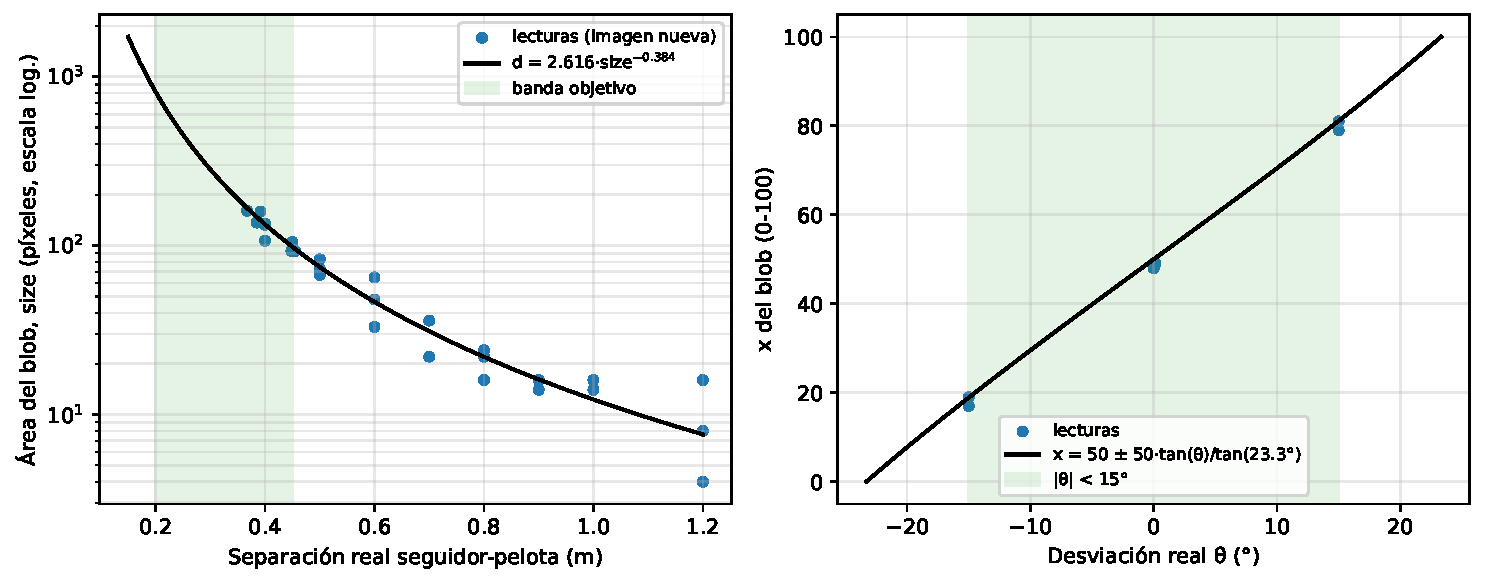
\includegraphics[width=\linewidth]{caracterizacion.pdf}
\caption{Caracterización estática del detector: seguidor colocado a distancias y rumbos conocidos, una imagen
nueva por posición. Izquierda: área del blob frente a la separación real y modelo ajustado
$d=2{,}616\cdot\text{size}^{-0{,}384}$. Derecha: $x$ del blob frente a la desviación real y modelo de cámara
estenopeica con un campo de visión de 46,6°.}
\label{fig:caract}
\end{figure}

\begin{figure}[h]
\centering
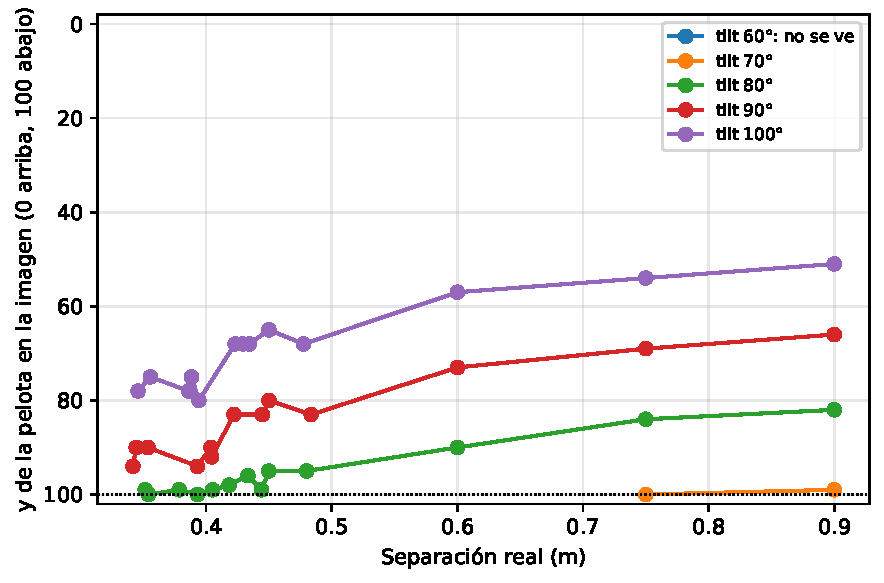
\includegraphics[width=0.6\linewidth]{barrido_tilt.pdf}
\caption{Altura de la pelota en la imagen frente a la separación para cada inclinación de la cámara. Con 100° se
ve en todo el rango de separaciones de interés.}
\label{fig:tilt}
\end{figure}

\subsection*{A2. Hiperparámetros}
\textbf{SAC:} \cod{learning\_rate} $3\cdot10^{-4}$, \cod{buffer\_size} 100\,000, \cod{learning\_starts} 1000
(calentamiento de avance), \cod{batch\_size} 256, $\tau$ 0,005, \cod{train\_freq} 1, \cod{gradient\_steps} 1,
coeficiente de entropía automático, $\gamma$ 0,99. \textbf{PPO:} \cod{learning\_rate} $3\cdot10^{-4}$,
\cod{n\_steps} 512, \cod{batch\_size} 64, \cod{n\_epochs} 10, $\lambda_{\text{GAE}}$ 0,95, \cod{clip\_range} 0,2,
\cod{ent\_coef} 0, $\gamma$ 0,99. Redes MLP por defecto de SB3 en ambos.

\subsection*{A3. Curvas de aprendizaje de C2}
Todas las curvas se generan con \cod{p1\_curvas.py} a partir del \cod{monitor.csv} de cada entrenamiento. Eje
horizontal: pasos del entorno. Media móvil de 10 episodios y, en trazo tenue, la serie sin suavizar. La línea
discontinua es la recompensa media por episodio de la política aleatoria en el entorno de entrenamiento (3,3).
El último panel o los dos últimos dan el porcentaje de episodios que terminan por cada causa (\cod{tiempo} =
completado).

\begin{figure}[p]
\centering
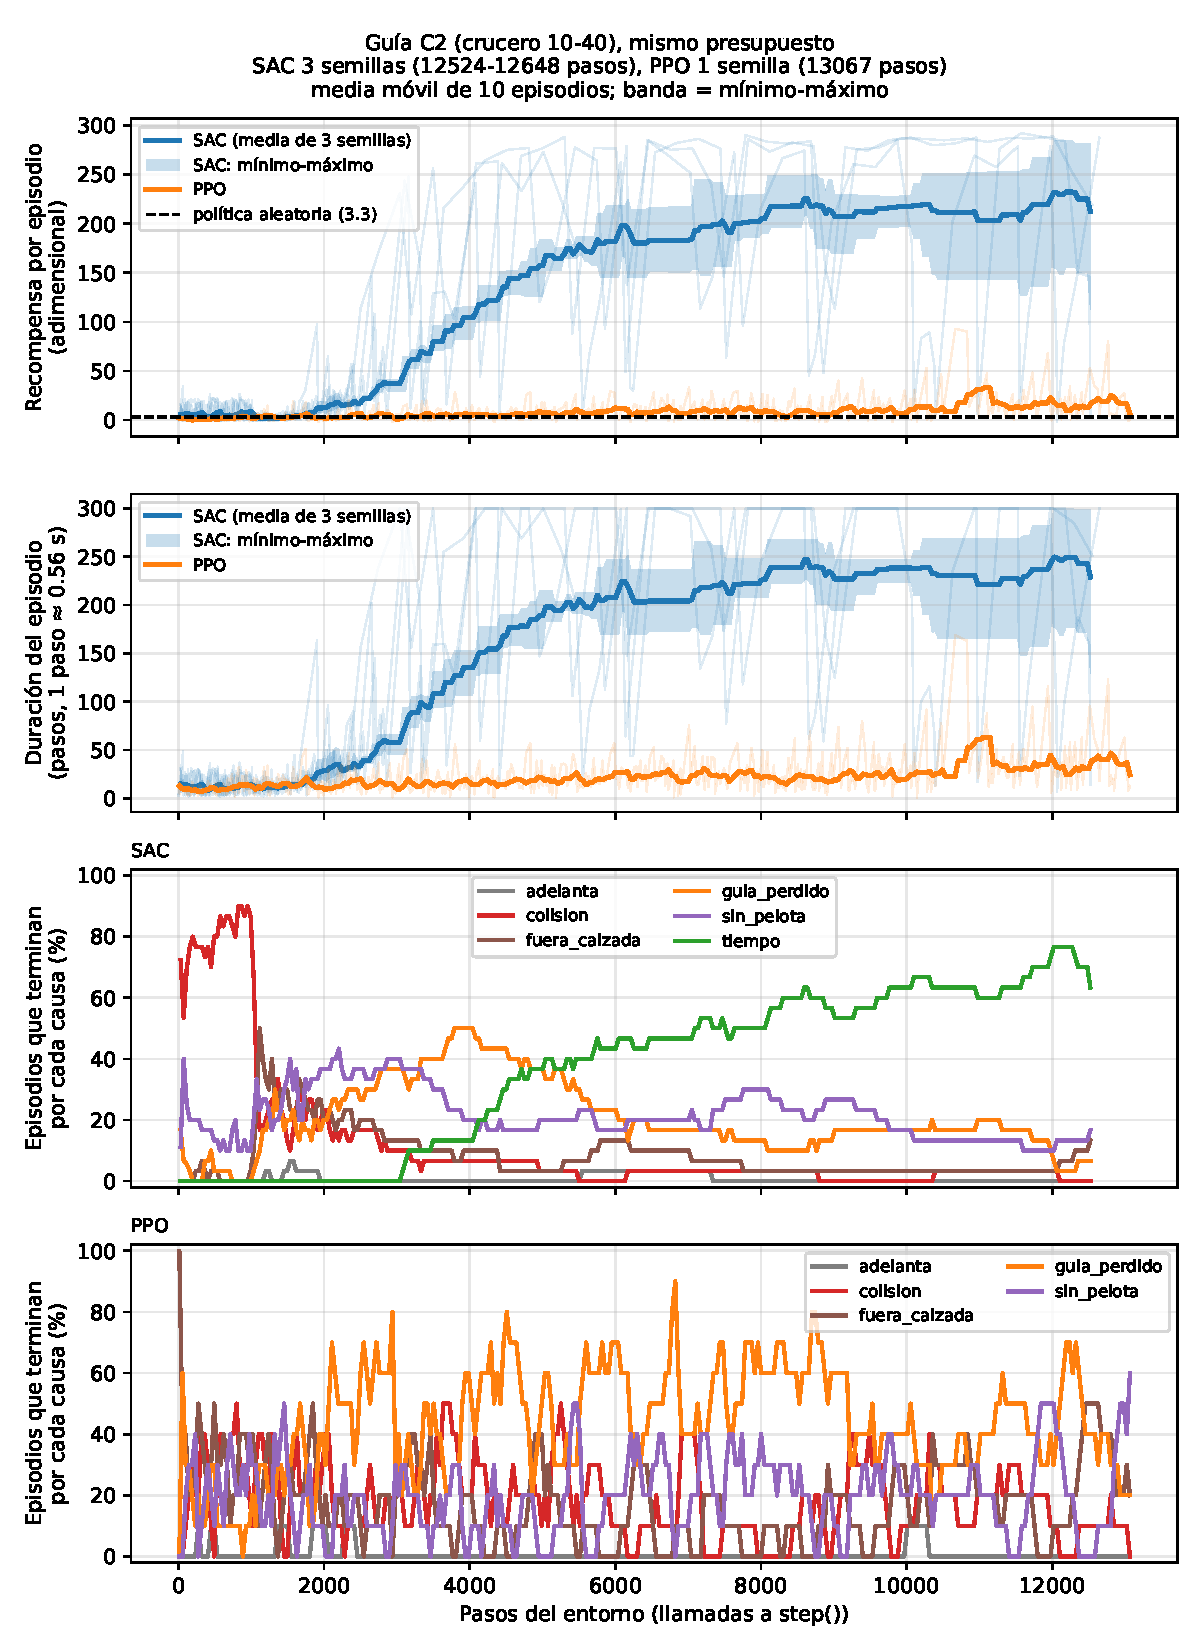
\includegraphics[height=0.86\textheight]{curvas_C2.pdf}
\caption{C2 (crucero 10--40), mismo presupuesto: SAC con 3 semillas (media y banda mínimo--máximo; 12\,524--12\,648
pasos) y PPO con 1 semilla (13\,067 pasos). Ventana de 10 episodios; 1 paso $\approx$ 0,56~s.}
\label{fig:curvasC2}
\end{figure}

\begin{figure}[p]
\centering
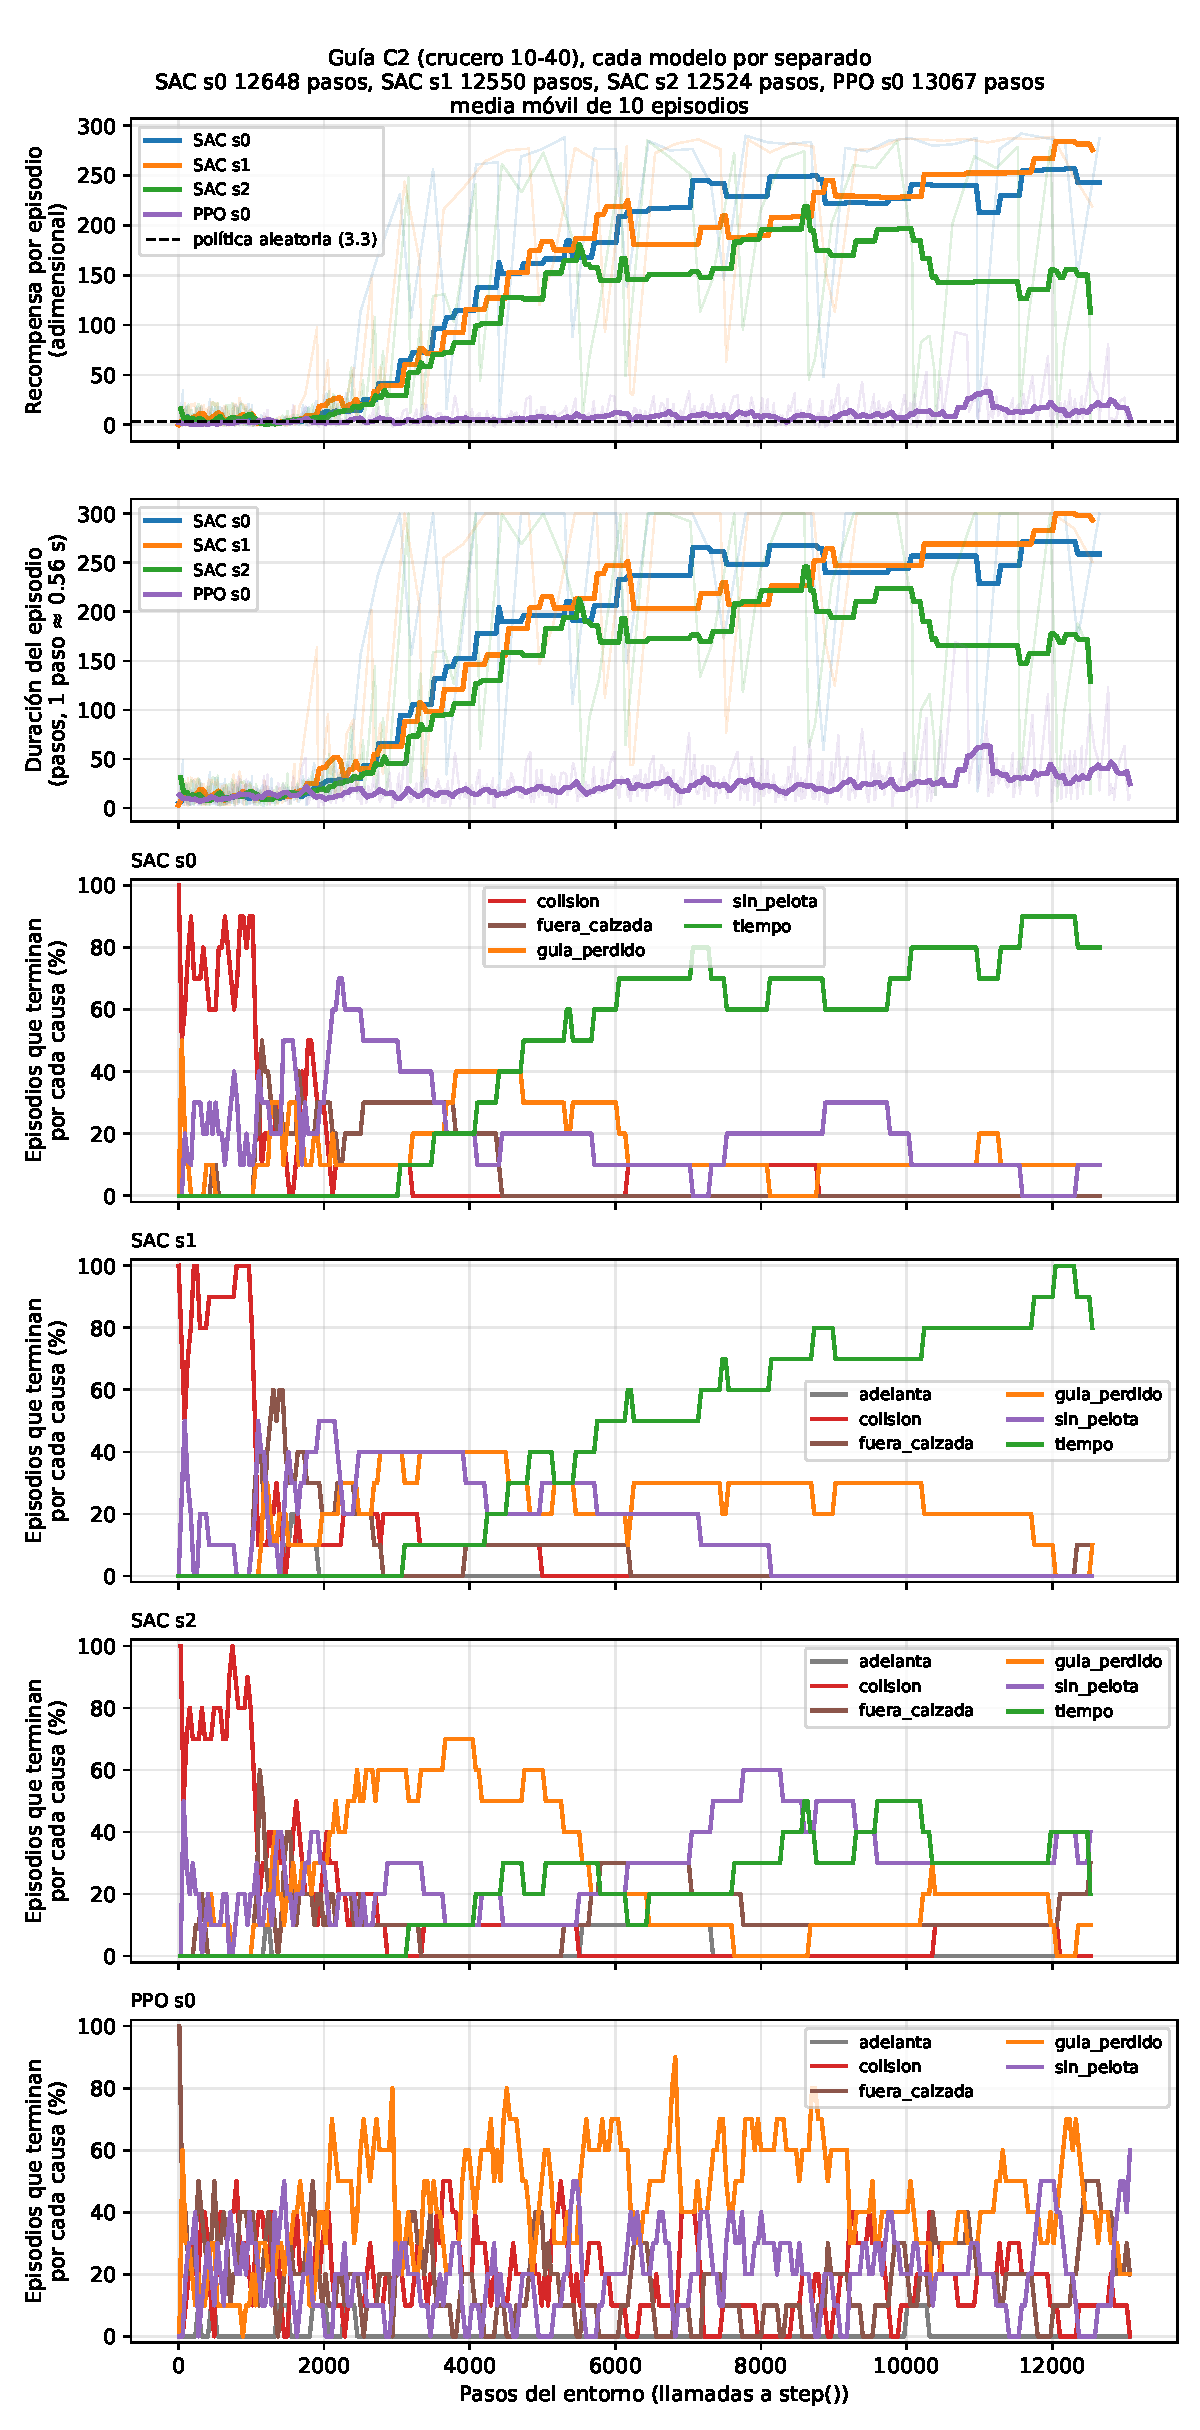
\includegraphics[height=0.86\textheight]{curvas_C2_modelos.pdf}
\caption{C2, cada modelo por separado (SAC s0, s1 y s2, y PPO s0), con el mismo presupuesto. Ventana de 10
episodios.}
\label{fig:curvasC2mod}
\end{figure}

\begin{figure}[p]
\centering
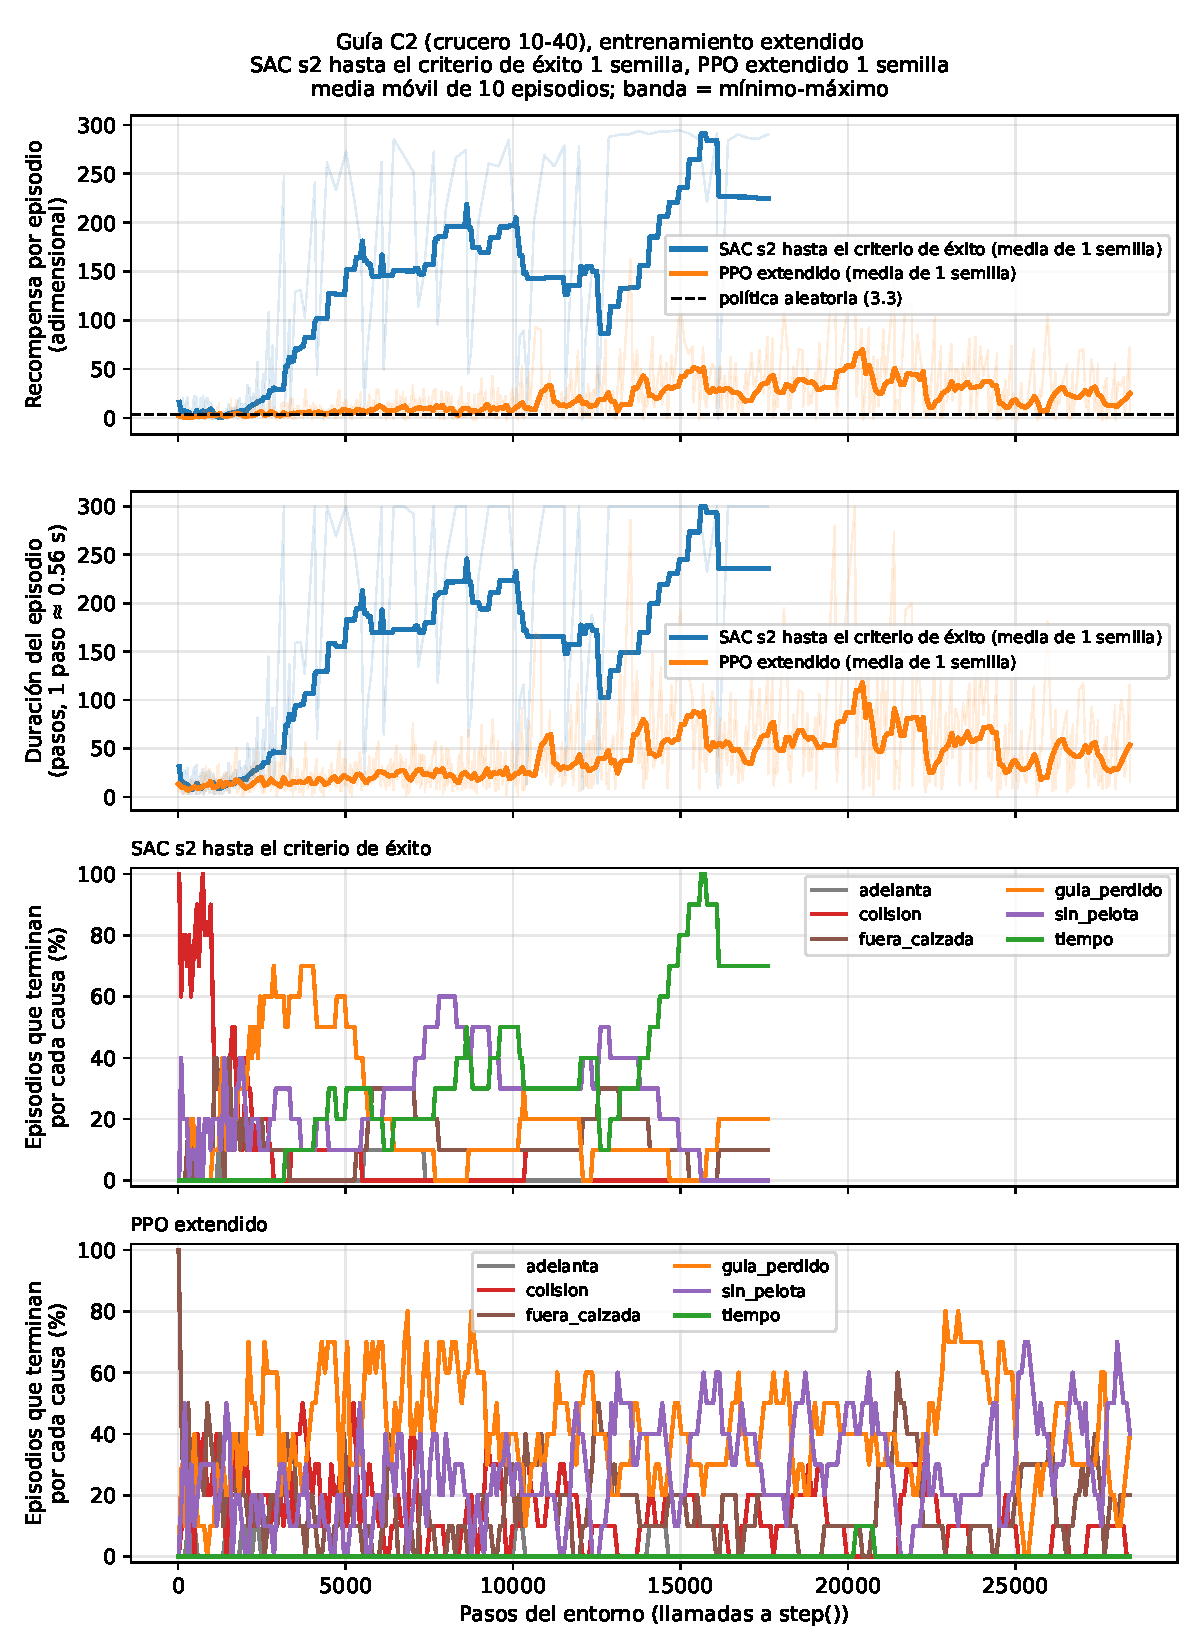
\includegraphics[height=0.86\textheight]{curvas_C2_ext.pdf}
\caption{C2, entrenamientos extendidos: SAC s2 hasta cumplir el criterio de éxito (17\,616 pasos) y PPO s0 con más
del doble de presupuesto (28\,421 pasos). 1 semilla cada uno. Ventana de 10 episodios.}
\label{fig:curvasC2ext}
\end{figure}

\subsection*{A4. Transferencia al robot real}
\pendiente{caracterización en el robot real y resultados}. Todo lo que depende de la calibración está en
\cod{p1\_config.json}: modelo de distancia ($k$, $p$), campo de visión, inclinación, factores de velocidad e IR.
La observación usa magnitudes físicas (metros, m/s) para que, tras repetir \cod{--caracterizar} y
\cod{--calibrar-movimiento} en el robot real, signifique lo mismo que en simulación. La política se ejecuta sin
simulador, con el reinicio a cargo de una persona (\cod{--ejecutar --sin-simulador}).

\end{document}
